% !TeX root = ../main.tex
% Add the above to each chapter to make compiling the PDF easier in some editors.

\chapter{Research}\label{chapter:research}

\section{Inspiration}
The concept of text adventures, choice based games or gamebooks is by far not new, and dates back long before electrical computers were even invented. They are a type of game that work almost inherently well on any type of device capable of displaying text and accepting input, as that in its most basic form is all they need. However, the question with every type of device remains how that is done intuitively and most true to the user's preferred consumption method with that device. With modern smartphones and tablets, the most popular input methods are tapping and swiping, and extensions of those to perform more complex actions. For a text adventure, this is contrast to the classic physical typing on a keyboard or even the pointing and clicking with a mouse. As such, it is clear a mobile text adventure ideally adapts and adopts tapping and swiping. In the spirit of the aforementioned game genres, that means swiping through texts or other forms of content and tapping items, replies or similar. 
Another aspect of these types of games has always been the deliberate lack of visual stimuli. Much like the classic understanding of books, they aim to elicit purely imaginary experiences. The user should mentally picture the events, draw their own version of the world, and not be bound to an artist's specific interpretation. 
One game in particular that we think captures the essence of these two sides very well is the Lifeline series of games developed by Three Minute Games in 2015 and 2016 for Apple iOS and Google Android\cite{LIFE}. The player is confronted with an at the beginning unknown world and one character. Descriptions of the world and events are delivered through the eyes of that character, and all the player can sometimes do is choose between two replies to a prompt by the character. Despite this simplicity, through the course of the game, the player envisions the entire world, the looks, the events and everything as they see fit. At the same time, the game is simple enough to be played even while being mobile with a smartphone in hand and does not require constant attention. 
This sparked the question about what options are available nowadays for creating this type of game. As looking at related work showed, the readily available options are often lackluster, but also provide valuable insight into what features need to be combined into one tool to provide satisfying overall functionality to both inexperienced and experienced user groups.

\section{Related work}
When analyzing related work, several categories were sampled. For one other popular text adventure games, both mobile and web based, to see what resonates well with audiences so far. Secondly other frameworks designed for the same or similar purposes, creating text adventures, to see what feature sets are available and seen as worthwhile by developers. Lastly, several specialist literary works on interactive storytelling, serious games and usability. Additionally, some functionality was deduced through logical inference and, frankly, common sense, since some basic features are simply necessary for such a framework to function at all.
Whenever a game was analyzed, a list of relevant features was extracted and matched up with the existing feature list in order to determine which additions or changes may need be made.

\subsection{Games}

\paragraph{Lifeline} 
The first game analyzed was Lifeline by Three Minute Games on iOS, as it also posed as main inspiration for the thesis. What can be seen in the game is that simplicity is key when aiming for accessibility with a large user group of smartphone users of all skill levels. Lifeline offers a simple structure of 1:1 communication between the player and one game character through a sequential text message stream. The interactive part for the player is reduced to the ability of choosing one of two replies when prompted by the game character every few messages. 
The story is acted out in real time, or rather with 1:1 time scaling. When the character claims to need several hours for an action, the game will accurately remain inactive for that long and only notify the player once as much time has passed.
A brief settings menu allows trivial changes such as toggling sounds and music, changing language, and more relevant to the game, to rewind the story to a previously reached decision and to speed up the gameplay by way of reducing UI effects and animation. 
The player can always scroll back through the entire story and through these settings choose a particular previous state once they have completed one story branch. 
What could be gathered from Lifeline is that ConText would need at least a basic dialogue system with multiple reply options offered to the user and possibly timed firing, as well as a mechanism to save new and load existing story progress. Additionally, it would need to provide at least a simple UI with potential customization for the user, as well as possibly settings for language support, sounds and the UI. \cite{LIFE}

\begin{figure}[!h]
\centering
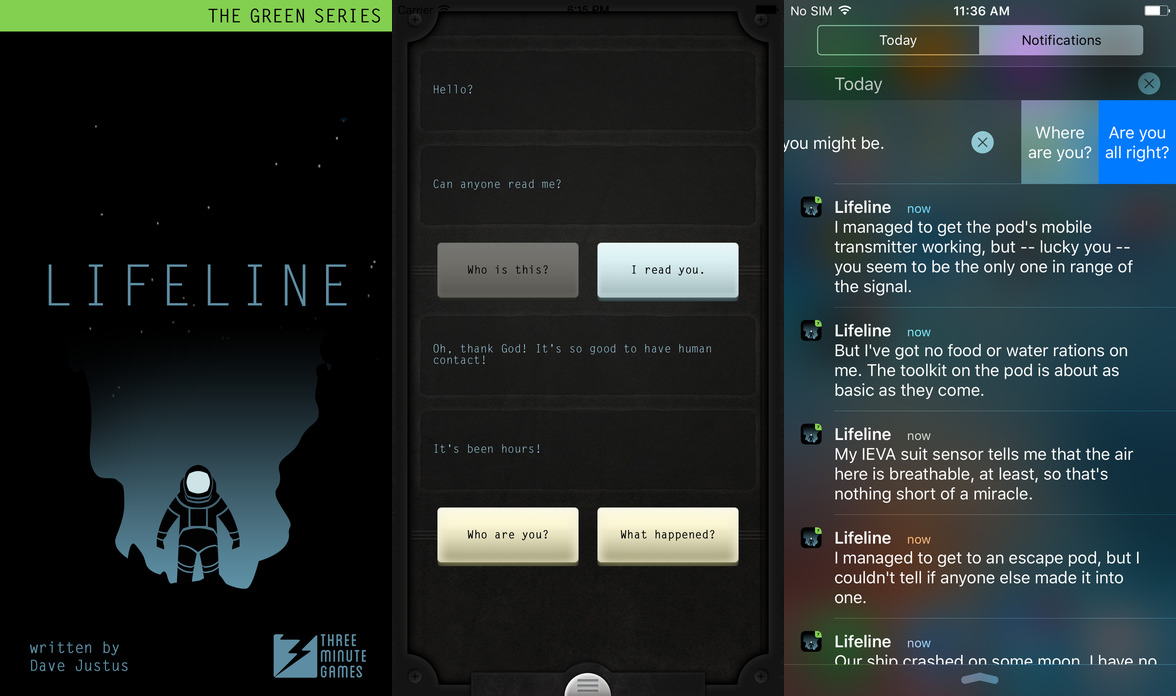
\includegraphics[width=0.85\textwidth]{figures/lifeline.png}
\caption[Lifeline (iOS)]{Lifeline, title screen, text stream and notifications side by side, as on \cite{LIFEiOS}.}\label{fig:lifeline}
\end{figure}

\paragraph{Storynexus.com} 
Another sample was taken from a web based service called storynexus.com. Storynexus is a website where users can create and more prominently play text adventures through their web browser. The story 'The Thirst Frontier' was chosen for analysis. It is mostly reminiscent of choice adventures or choose-your-own-adventure stories in that the user is guided through a story with partially branching story arcs and with every new page is asked to choose from available options that can include virtual actions or dialogue replies. The story is segmented into locations or chapters of sorts. While it does not offer 1:1 time scaled playback as Lifeline, it does stand out through a more complex item and character quality system that can additionally influence the success of attempted actions or their mere existence. 
This analysis expands the list of viable features for ConText by a system for splitting the story into chapters, which may not reflect in the created App but for clarity in the framework interface. As a possible secondary feature it promotes extended player properties that influence and are influenced by how the story unfolds, as well as a dedicated inventory for items to be used in gameplay actions. \cite{SNEXUS}\cite{SNEXTTF}

\begin{figure}[!h]
\centering
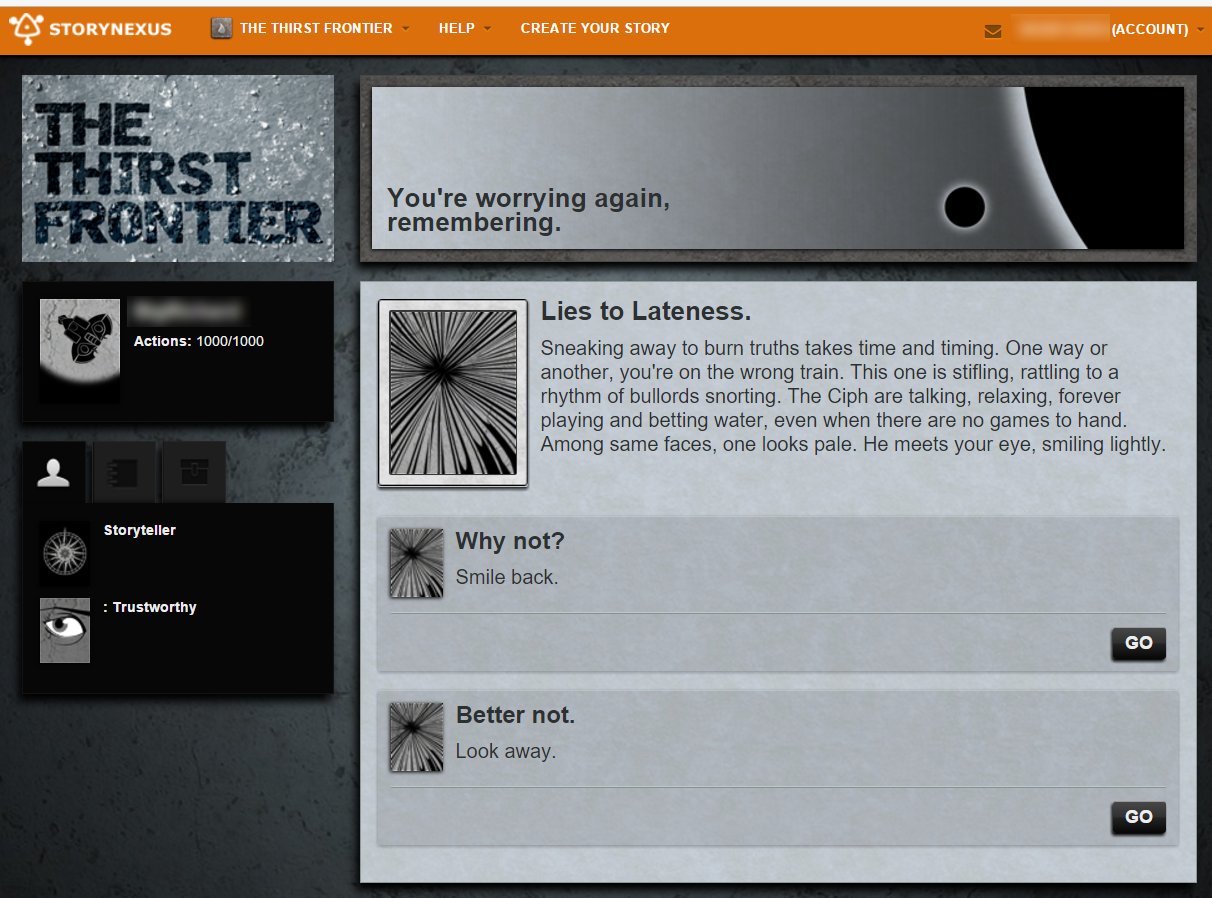
\includegraphics[width=0.85\textwidth]{figures/storynexus.png}
\caption[Storynexus.com; The Thirst Frontier]{An early page in The Thirst Frontier available on Storynexus.com, as on \cite{SNEXTTF}.}\label{fig:storynexus}
\end{figure}

\paragraph{Ludus} 
A prime candidate for consideration was TUM student Moritz Becher's \textit{Ludus}, another Bachelor's Thesis building on a very similar topic as this one. Ludus is a mobile text adventure game set in ancient Rome and designed to teach the player historical facts about the setting. It was actually developed under the same supervisor and for the same overall topic of educational serious games. The game itself was not directly analyzed, instead Becher was contacted and asked about his ideas on what features this framework would need and which features he deemed useful for his project. As a result, some of his concepts for internal structures such as the decoupling and communication of story and user interface served as inspiration for some of ConText's systems. Over the course of development the framework actually diverged from these concepts again, however. Additionally, Becher participated in the second user study given his thesis essentially qualifies him as an expert on the subject. \cite{LUDUS}

\subsection{Frameworks}
\paragraph{Quest \& Squiffy} 
Both Quest and Squiffy are web based frameworks for creating text adventures, gamebooks and interactive fiction. The focus seems to lie on straight forward creation of these types of games with a high level of compatibility with devices due to the reliance on entirely web based technology like HTML and JavaScript. With Quest, a simple result is easy to achieve, with scripting language integration available should users want to add specific functionality. In these aspects, it is very akin to what ConText aims to be. The downside is, however, that the feature expansion is limited to what HTML and JavaScript can do within the confines of the tools and should the user want to integrate functionality outside of the typical scope of a website, they are confronted with a large amount of custom scripting. \cite{QUEST}
Squiffy is locked down to the specific markup and scripting language used in the tool, but also promises quick results.
Both tools need additional tools to encapsulate a story into a standalone app. 
Experimenting with Quest and Squiffy did provide a better understanding of the properties the module types would need such as names, types, content, linking options and possible actions as well as a better idea of the scope of the framework that is needed for a basic system and viable for the temporal terms of this thesis. \cite{SQUIFFY}
\paragraph{Other}
Other tools such as Inform\cite{INFORM}, a natural language based system, WibbleQuest\cite{WIBBLE}, a library for developing iOS text adventures or ADRIFT\cite{ADRIFT}, a graph based text adventure creator were all briefly considered but not analyzed in more detail as the already listed sources of inspiration as well as some specialist literature and aforementioned logical inference provided enough aspects and features to define ConText's core concept and structure design. 
One downside that was common to all regarded toolkits was the comparably lackluster expansion capabilities, with some supporting extenions within the limits of their base systems, but none as potentially diverse and simultaneously viable solutions as Unity engine's.

\subsection{Literature}
Specialist literature was used to help determine what other international projects and papers deem necessary or beneficial to watch out for when creating tools designed to create text adventures. 
\paragraph{On E-Learning and Interactive Storytelling technology}
In order to get such an idea specifically related to educational and serious games, proceedings from several conferences on the topic were consulted. In one such volume from \cite{ELEARN}, Danu Pranantha et al. while developing a HTML5 framework for creating serious games suggest categorization of serious game creation tools and their development into \glqq 1) the development of platform for ease to use game creation using pre-created game props 2) the use of advanced web technologies to develop browser games which offers cross platform capability\grqq (sic!)\cite{ELEARN1}. Additionally, they acknowledge in the prior sentence that game engines exist and can serve as a base platform for such tools. Thus, ConText could be categorized as following approach 1 while using Unity engine as a base. In that same sentence, Pranantha et al. also raise concerns about the cross platform capabilities and issues of using an existing engine, which we deem outdated at this point, however, as in the four years between the proceedings and this thesis, cross platform capabilities of the Unity engine have been greatly improved and verified to work well in conjunction with ConText's features and a deployed game created with it in an internal test. Overall, similar categorization is also suggested by various other efforts in the consulted material and ConText fits as a plugin system for a widely available existing game engine. The advantages of this design are that the low level components such as rendering, input handling, etc. are covered, that a large community as well as detailed documentation are available and that through this community, some potential users are easier to reach. 
Diving into proceedings on interactive storytelling also yielded some helpful directions, in the case of \cite{ISTORY} and \cite{ISTORY1} specifically on user experience testing. While the paper itself actually targets methods for successful story authoring, one key point is user experience, that "The User Experience is crucial". In it, Koenitz writes that user studies should deliberately "cast the net as wide as possible and try to avoid techno-savvy users"\cite[p.~135]{ISTORY} as those do not already appreciate the studied artifact for technical aspects but instead judge from the viewpoint of someone without preexisting knowledge and as such more akin to the common average user. This also promises to bring more attention to lackluster UI simplicity as these users would not be as used to complex interfaces.

The overall experience when looking for adequate literature touching the topic of (serious) text adventures, frameworks for the creation of such and the requirements and best practices proved lackluster and suggests that the subject has been somewhat unpopular until now and a lot of groundwork has yet to be covered or publicly and widely shared. As described earlier, plenty of functionality of ConText has been designed based on logical needs and common sense dictated by the planned feature set. 
\paragraph{On usability and user experience}
The two topics usability and user experience were given low priority until a functional prototype was set up and the majority of planned features were implemented, as such only some research was done, particularly when the user studies were conducted. 
For one to better figure out which aspects of the framework to categorize and evaluate through the studies, but also to determine how to change parts flawed in terms of usability between and after the studies. 

A paper by Cristian Rusu et al. called "User Experience Evaluations: Challenges for Newcomers" in \cite{DUXU} provided a very useful rundown of major concepts and principles for testing usability and user experience. With the definition of usability found in ISO 9241 - "the extent to which a system, product or service can be used by specified users to achieve specified goals with effectiveness, efficiency and satisfaction in a specified context of use" \cite[p.~237]{DUXU1}\cite{UISO} - one can already distinguish the metrics effectiveness, efficiency and satisfaction that need to be maximized to achieve better usability, also called the summative approach. On the other hand Rusu further explains the formative approach which classifies evaluation methods to facilitate "usability problems detection" and solutions, the two main methods being "empirical usability testing, based on users' participation" and "inspection methods, based on experts' judgment" \cite[p.~240]{DUXU1}. 
These methods could thus be used to detect and solve usability problems where the solutions would in turn optimize the summative metrics. For the user studies in this thesis, the empirical method was chosen. 

Once usability optimization was an active agenda task, works on the topic were consulted, most notably Steve Krug's "Don't Make Me Think - Revisited" \cite{DMMThink}. While the book is overall intended to inform about web usability, the core principles explained in it apply to programs and some usability problems in general as well. Krug's definition of usability is that "A person of average (or even below average) ability and experience can figure out how to use the thing to accomplish something without it being more trouble than it's worth" \cite[p.~9]{DMMThink}. When looking at how to improve usability for a tool, the two of his four primary suggestions that are most viable in a small scope are "\#{}1. Fix the usability problems that confuse everyone", which were to be determined by the user studies and "\#{}2. Go for the low-hanging fruit", essentially meaning to focus on issues that can be resolved more quickly and thus in a greater number instead of issues that take more effort to fix while possibly not providing much improvement \cite[p.~178-180]{DMMThink}.

More in-depth literature such as Jakob Nielsen's 10 Usability Heuristics and evaluation \cite{NNG} were considered but ultimately disregarded as the scope of this thesis proved to be too narrow to incorporate larger scale usability testing.
